\section{Business Process Model and Notation (BPMN)}\label{sec:bpmn}

\ac{BPMN} ist ein Standard zur Modellierung von Geschäftsprozessen. Die Notation wurde entwickelt, um eine einheitliche Notation bereitzustellen, die sowohl von Geschäftsanalysten als auch von technischen Entwicklern verstanden wird. \ac{BPMN}-Modelle bestehen aus verschiedenen Elementen wie Aktivitäten, Ereignissen, Gateways und Verbindungen, die zusammen den Ablauf eines Geschäftsprozesses darstellen \cite{omgbpmn}.

\subsection*{Relevante BPMN-Elemente}
Für die Identifikation von \ac{DSGVO}-kritischen Aktivitäten sind insbesondere folgende Elemente relevant, da sie Hinweise auf den Umgang mit (personenbezogenen) Daten geben:

\begin{itemize}
    \item \textbf{Aktivitäten}: bilden die auszuführenden Arbeitsschritte eines Prozesses ab. Sie können Ein- und Ausgaben sowie Datenabhängigkeiten definieren \cite{omgbpmn}. Durch ihren Namen oder Kontext können Rückschlüsse auf die Verarbeitung personenbezogener Daten gezogen werden.
    \item \textbf{Sequenzflüsse}: verbinden Aktivitäten, Ereignisse und Gateways und zeigen die Reihenfolge der Ausführung im Prozess an \cite{omgbpmn}. Mit ihrer Hilfe kann eine einzelne Aktivität im Kontext des gesamten Prozesses betrachtet werden, indem der Pfad zu und von der Aktivität verfolgt wird.
    \item \textbf{Datenobjekte und Datenspeicher}: repräsentieren flüchtige oder persistente Daten, die im Prozess von z.B. Aktivitäten genutzt oder geschrieben werden können \cite{omgbpmn}. Sie können auch personenbezogene Daten enthalten.
    \item \textbf{Datenassoziationen}: Eingangs- und Ausgangsassoziationen verbinden Aktivitäten mit Datenobjekten und Datenspeichern und zeigen so Ein- und Ausgaben explizit an \cite{omgbpmn}. Sie sind ein wichtiges Signal für die Verarbeitung personenbezogener Daten, da sie den direkten Bezug einer Aktivität zu bestimmten Daten verdeutlichen (z.B. Lesezugriff auf eine Kundendatenbank).
    \item \textbf{Pools und Lanes}: Pools modellieren Organisationseinheiten oder Prozessbeteiligte, während Lanes Verantwortlichkeiten innerhalb eines Pools darstellen. Innerhalb eines Pools befinden sich die Aktivitäten und anderen Elemente des Prozesses \cite{omgbpmn}. Die Rollen und Verantwortlichkeiten, die durch Pools und Lanes dargestellt werden, können für die Bewertung der Datenverarbeitung relevant sein.
    \item \textbf{Nachrichtenflüsse}: stellen den Austausch von Nachrichten zwischen verschiedenen Pools dar \cite{omgbpmn}. Sie können auf eine Übermittlung personenbezogener Daten an Dritte hinweisen (z.B. Transfer von Kundendaten an einen externen Dienstleister).
    \item \textbf{Textannotationen und Assoziationen}: dienen dazu, zusätzliche Informationen zu Prozessmodellen hinzuzufügen, die nicht durch die standardmäßigen BPMN-Elemente abgedeckt sind \cite{omgbpmn}. Sie können genutzt werden, um die Art der Datenverarbeitung zu präzisieren (z.B. „enthält E-Mail-Adresse“).
\end{itemize}

\subsection*{\ac{BPMN}-XML}

\ac{BPMN}-Modelle werden in einer XML-Serialisierung gespeichert (\ac{BPMN} 2.0 XML) \cite{omgbpmn}. Diese Darstellung enthält alle relevanten Strukturinformationen (Elementtypen, Namen, Beziehungen, Zuordnungen, Positionen der Elemente) und wird von vielen Prozess-Engines und Modellierungswerkzeugen wie Camunda \cite{camunda} und BPMN.io \cite{bpmnio} unterstützt. Für diese Arbeit dient \ac{BPMN}-XML als Eingabeformat der Klassifizierungspipeline (siehe Kapitel \ref{ch:klassifizierungsalgorithmus-(design-und-implementierung)}).

Im Metamodell von \ac{BPMN} erben fast alle Elemente von \texttt{BaseElement} und damit ein \texttt{id}-Attribut. Dieses \texttt{id} dient der eindeutigen Referenzierung und ist \emph{erforderlich} \cite{omgbpmn}. Diese ID ist für die Klassifizierungspipeline wichtig, da sie eine stabile Referenzierung der Aktivitäten und anderer Elemente ermöglicht. Dies ist insbesondere dann relevant, wenn die Ergebnisse der Klassifizierung auf die ursprünglichen Prozessmodelle zurückgeführt werden müssen.

\subsection*{Beispiel einer Datenassoziation als Datenschutzsignal}

\begin{figure}
    \centering
    \begin{subfigure}{.5\textwidth}
        \centering
        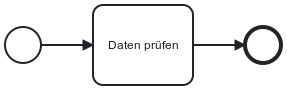
\includegraphics[width=.7\linewidth]{images/process-models/data-association-example-uncritical}
        \caption{Ohne Datenassoziation}
        \label{fig:without-data-association}
    \end{subfigure}%
    \begin{subfigure}{.5\textwidth}
        \centering
        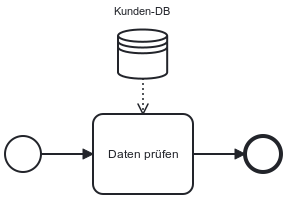
\includegraphics[width=.7\linewidth]{images/process-models/data-association-example-critical}
        \caption{Mit Datenassoziation}
        \label{fig:with-data-association}
    \end{subfigure}
    \caption{ Beispiel einer Datenassoziation als Datenschutzsignal.}
    \label{fig:data-association-gdpr-example}
\end{figure}

Abbildung \ref{fig:data-association-gdpr-example} zeigt ein einfaches Beispiel, wie eine Datenassoziation die \ac{DSGVO}-Relevanz einer Aktivität verdeutlichen kann. In Abbildung \ref{fig:without-data-association} ist die Aktivität \enquote{Daten prüfen} ohne Datenassoziation dargestellt, was wenig über die Art der verarbeiteten Daten aussagt. In Abbildung \ref{fig:with-data-association} hingegen zeigt die eingehende Datenassoziation von einem Datenspeicher \enquote{Kunden-DB}, dass die Aktivität personenbezogene Daten verarbeitet. Dies macht die Aktivität als potenziell datenschutzkritisch erkennbar. Dieses Beispiel unterstreicht die Notwendigkeit den gesamten Kontext einer Aktivität zu betrachten, um fundierte Rückschlüsse auf die Verarbeitung personenbezogener Daten ziehen zu können.